\documentclass[border=6pt]{standalone}
\usepackage{tikz}
\usepackage[edges]{forest}
\usetikzlibrary{arrows.meta,positioning,calc,decorations.pathreplacing,shapes.geometric}
\begin{document}
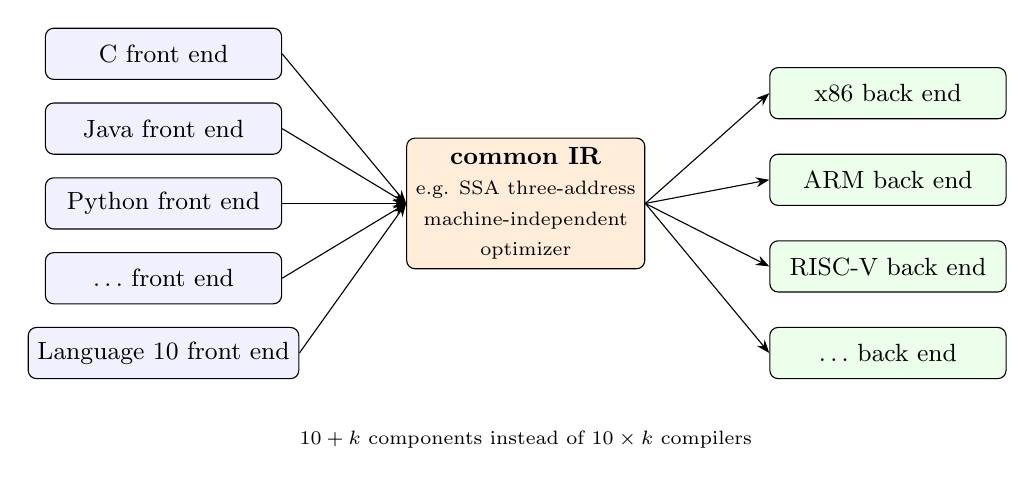
\begin{tikzpicture}[>=Stealth,font=\small,
 fe/.style={draw,rounded corners=3pt,fill=blue!6,minimum width=3.0cm,minimum height=0.65cm},
 be/.style={draw,rounded corners=3pt,fill=green!8,minimum width=3.0cm,minimum height=0.65cm}]
\node[fe] (f0) at (0,0.00) {C front end};
\node[fe] (f1) at (0,-0.95) {Java front end};
\node[fe] (f2) at (0,-1.90) {Python front end};
\node[fe] (f3) at (0,-2.85) {$\ldots$ front end};
\node[fe] (f4) at (0,-3.80) {Language 10 front end};
\node[be] (b0) at (9.2,-0.50) {x86 back end};
\node[be] (b1) at (9.2,-1.60) {ARM back end};
\node[be] (b2) at (9.2,-2.70) {RISC-V back end};
\node[be] (b3) at (9.2,-3.80) {$\ldots$ back end};
\node[draw,rounded corners=3pt,fill=orange!15,minimum width=2.6cm,minimum height=1.6cm,align=center] (ir) at (4.6,-1.9) {\textbf{common IR}\\{\scriptsize e.g. SSA three-address}\\{\scriptsize machine-independent}\\{\scriptsize optimizer}};
\foreach \i in {0,...,4} \draw[->] (f\i.east) -- (ir.west);
\foreach \i in {0,...,3} \draw[->] (ir.east) -- (b\i.west);
\node[font=\scriptsize] at (4.6,-4.9) {$10 + k$ components instead of $10 \times k$ compilers};
\end{tikzpicture}
\end{document}
